% CLiMB 2026 (EndoVis @ MICCAI 2026) -- final method write-up, team Jmees26.
% Body limited to 3 pages excluding references (challenge requirement).
% Build: bash build.sh
\documentclass[10pt,a4paper]{article}
\usepackage[margin=2.05cm]{geometry}
\usepackage{times}
% texlive-small ships Times but not Courier: keep CM typewriter
\renewcommand{\ttdefault}{cmtt}
\usepackage{amsmath,amssymb}
\usepackage{graphicx,booktabs,xcolor}
\usepackage[font=small,labelfont=bf,skip=3pt]{caption}
\usepackage{tikz}
\usetikzlibrary{arrows.meta,positioning,fit}
\usepackage[hidelinks]{hyperref}

\setlength{\parskip}{1pt}
\setlength{\textfloatsep}{6pt}
\setlength{\intextsep}{6pt}
\setlength{\abovedisplayskip}{3pt}
\setlength{\belowdisplayskip}{3pt}
\renewcommand{\arraystretch}{1.03}
% tighter section/paragraph spacing without titlesec (not in texlive-small)
\makeatletter
\renewcommand\section{\@startsection{section}{1}{\z@}%
  {5pt plus 2pt minus 1pt}{2pt}{\normalfont\large\bfseries}}
\renewcommand\paragraph{\@startsection{paragraph}{4}{\z@}%
  {3pt plus 1pt minus 1pt}{-0.55em}{\normalfont\bfseries}}
\makeatother

\newcommand{\TODO}[1]{\textcolor{red}{#1}}

\title{\vspace{-1.4cm}\bfseries Sub-map-aware feed-forward monocular SLAM for colonoscopy:\\
windowed Depth Anything 3 with fisheye field-of-view correction\\ and robust rotation averaging}
\author{Shunsuke Kikuchi, Atsushi Kouno, Ryosuke Goto, Hiroki Matsuzaki\\[1pt]
\small Jmees Inc., 5\mbox{-}4\mbox{-}6 Kashiwanoha, Kashiwa, Chiba, Japan\\
\small\texttt{engineer@jmees-inc.com}}
\date{}

\begin{document}
\maketitle
\vspace{-1.0cm}

\noindent\fbox{\parbox{\dimexpr\textwidth-2\fboxsep-2\fboxrule}{\small
\textbf{Team name:} Jmees26 \quad\textbullet\quad
\textbf{Synapse submission ID:} \textbf{9780121} (alias \texttt{v099}) \quad\textbullet\quad
\textbf{Leaderboard:} \texttt{climb\_score} \textbf{4.078}, rank 2 (1st place 3.559).\\
\textbf{Public release of this write-up:} \textbf{Yes} --- the authors agree to make this write-up public
and to the co-authorship terms of the challenge Publication Policy.\\
\textbf{Source code:} \url{https://github.com/JmeesInc/CLiMB26-jmees}
}}

\section{Background}
Colonoscopy breaks the assumptions of classical feature-based SLAM: the mucosa is texture-poor and
specular, the tissue deforms continuously, the light source is rigidly attached to the camera so
appearance changes with viewpoint, and the optics are a strongly distorted fisheye. On the
challenge's simulated sequences the official ORB-SLAM3 baseline~\cite{orbslam3} loses tracking and splits into
fragments, and its accuracy degrades monotonically with the amount of deformation
(1.11\,mm ATE at zero deformation, 16.21\,mm at maximum).

Our entry replaces the tracking/mapping front end entirely with a \emph{feed-forward multi-view
geometry foundation model}, Depth Anything 3 (DA3)~\cite{da3}, run on short overlapping windows and
chained in closed form --- no bundle adjustment, no loop closure, no keyframe graph. The pipeline is
deterministic and runs at 0.0197\,s/frame ($\approx$51\,fps) on the evaluation host.

The novelty is less in the backbone than in three findings that each moved the leaderboard by tens of
percent, and that we believe generalise beyond this challenge:
\textbf{(i)} the dominant error of a chained feed-forward reconstruction on real endoscopy is not
trajectory \emph{drift} but \emph{inter-window scale inconsistency}, which invalidates the usual
remedies (BA, pose graphs, loop closure) and makes the map \emph{granularity} --- how much of a clip
one claims to be a single metrically consistent map --- the correct lever;
\textbf{(ii)} feeding a rectified but extremely wide-angle pinhole image to a model that
self-estimates its own focal length shears rotation into translation, so the \emph{virtual}
field of view, not just the removal of distortion, has to be chosen;
\textbf{(iii)} because the evaluator's ATE uses only camera centres and RPE only orientations, the
rotations can be replaced wholesale by robust epipolar rotation averaging at zero ATE risk.

\section{Method}
Figure~\ref{fig:pipe} summarises the pipeline; each stage is described below.

\begin{figure}[t]
\centering
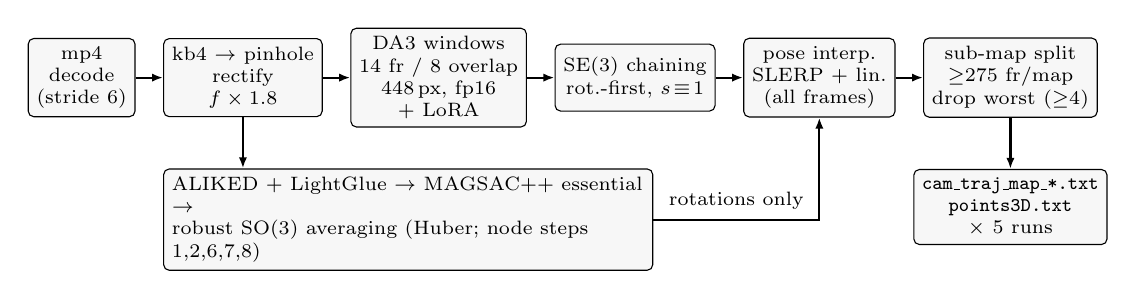
\begin{tikzpicture}[
  font=\scriptsize,
  box/.style={draw,rounded corners=2pt,align=center,inner sep=3pt,minimum height=8.5mm,fill=black!3},
  arr/.style={-{Latex[length=4pt]},thick}]
\node[box] (dec) {mp4\\decode\\(stride 6)};
\node[box,right=3.5mm of dec] (rect) {kb4 $\to$ pinhole\\rectify\\$f\times1.8$};
\node[box,right=3.5mm of rect] (da3) {DA3 windows\\14 fr / 8 overlap\\448\,px, fp16\\+ LoRA};
\node[box,right=3.5mm of da3] (chain) {SE(3) chaining\\rot.-first, $s\!\equiv\!1$};
\node[box,right=3.5mm of chain] (interp) {pose interp.\\SLERP + lin.\\(all frames)};
\node[box,right=3.5mm of interp] (split) {sub-map split\\$\geq$275 fr/map\\drop worst ($\geq$4)};
\node[box,below=6.5mm of rect.south west,anchor=north west,align=left,text width=60mm] (rot)
  {ALIKED + LightGlue $\to$ MAGSAC++ essential $\to$\\
   robust SO(3) averaging (Huber; node steps 1,2,6,7,8)};
\node[box,below=6.5mm of split.south,anchor=north] (out)
  {\texttt{cam\_traj\_map\_*.txt}\\\texttt{points3D.txt}\\$\times$ 5 runs};
\draw[arr] (dec)--(rect); \draw[arr] (rect)--(da3); \draw[arr] (da3)--(chain);
\draw[arr] (chain)--(interp); \draw[arr] (interp)--(split);
\draw[arr] (split.south)--(out.north);
\draw[arr] (rect.south)--(rot.north -| rect.south);
\draw[arr] (rot.east) -- node[above,font=\scriptsize]{rotations only} (rot.east -| interp.south) -- (interp.south);
\end{tikzpicture}
\caption{Pipeline. Everything is feed-forward and deterministic; the only learned adaptation is a
11.8\,MB LoRA adapter on the DA3 backbone. Rotation averaging modifies orientations only and leaves
camera centres bit-identical, so it cannot affect ATE.}
\label{fig:pipe}
\end{figure}

\paragraph{Pre-processing.}
Frames are decoded sequentially from the \texttt{mp4} with OpenCV; only every 6th frame is decoded
(non-keyframes are skipped with \texttt{cap.grab()}), which is both a $6\times$ speed-up and, on real
data, a $38\%$ ATE reduction because fewer windows mean fewer inter-window seams. Each keyframe is
undistorted from the Kannala--Brandt \texttt{kb4} model~\cite{kb} to a virtual pinhole. The
calibration is selected per sequence from the 18 official endoscope calibrations baked into the
image, using the public sequence$\to$endoscope metadata (challenge-provided; 75/93 sequences
covered), falling back to the mean calibration otherwise. Rectifying with \texttt{balance}$=0$
retains the full $111^\circ$ field of view; because DA3 self-estimates focal length and does so at
$1.6$--$2.5\times$ the true value on such images, we scale the virtual focal length by $1.8$
($\approx72^\circ$ FOV) at zero computational cost, which alone cut real-clip ATE from 4.08 to
3.35\,mm.

\paragraph{Windowed reconstruction and chaining.}
DA3 (\texttt{DA3NESTED-GIANT-LARGE}, 1.40B parameters) is run under \texttt{torch.no\_grad} on
windows of 12 keyframes with 6 shared frames, at 448\,px longest side in fp16. Each call returns
window-local poses and metric depth. A window is mapped into the global frame by a rigid transform
fitted on the shared cameras: rotation from the camera \emph{orientations}
($R=\Pi_{SO(3)}\sum_i R^{\text{glob}}_i R^{\text{loc}\top}_i$; a centres-only fit is ill-conditioned
because forward colonoscopy motion puts the centres on a near-straight line), translation from the
centroids, and \textbf{scale fixed at 1}. Estimating a per-window scale is measurably harmful
(5.25\,$\to$\,7.09\,mm with a clamped robust estimator, 19.27\,mm with plain least squares). Poses for
the skipped frames are filled by SLERP/linear interpolation, so every frame is output and TFR stays
at 100\%. The sparse map is the confident depth (above the 40th confidence percentile, on an 8-px
grid, from every 4th keyframe, capped at 200k points with a fixed seed) unprojected into the global
frame.

\paragraph{Rotation averaging.}
RPE$_{\text{rot}}$ depends only on trajectory orientations and ATE only on centres, so orientations can
be improved independently. On rectified keyframes (0.25 scale, 512 keypoints) we extract
ALIKED~\cite{aliked} features, match with LightGlue~\cite{lightglue}, and estimate a relative rotation
per edge with a MAGSAC++~\cite{magsac} essential matrix followed by \texttt{recoverPose}. Nodes are
placed every 6 frames and edges span $\{1,2,6,7,8\}$ nodes, so long edges measure the $\delta=40$
quantity \emph{directly} instead of accumulating it. Feature edges (weight = inlier count, two
rejection rounds) are fused with the DA3 edges (constant weight, the fallback where matching fails)
in a Huber-robust Gauss--Seidel SO(3) averaging~\cite{rotavg} with 30 sweeps; the early stop acts as a
regulariser. Camera centres are preserved exactly.

\paragraph{Sub-map partitioning.}
The evaluator aligns \emph{each} sub-map to the COLMAP reference with its own Sim(3), averages the
per-map ATEs weighted by matched poses, and \emph{sums} \texttt{ratio\_loc\_frames}. A disjoint
partition therefore scores each map over a span short enough that accumulated error has not
dominated. Across our leaderboard entries the per-clip ATE follows a power law in the realised map
span with exponent $\approx$0.9--1.2 (e.g.\ 4.76 at a mean span of 387 frames, 4.31 at 366,
3.91 at 313), so shorter maps are strictly better---until a map stops being scored. The scorer
counts a sub-map only if it shares at least \textbf{250} frame IDs with the reference (the
public evaluator still says 100; the leaderboard settles it: 200-frame maps score nothing on any
clip, 280-frame maps lose 4 clips, 380-frame maps none). The floor therefore has to be set as an
\emph{absolute} minimum span, independent of the target map count: we emit
$n=\mathrm{round}(N/260)$ maps and shrink $n$ until every map spans $\geq$275 frames, which gives
275--330-frame maps on typical clips. One test clip has a reference so sparse that it needs
$\geq$380-frame maps to be scored at all; its frame count is visible at inference, so we located it
by bisection on the leaderboard (three submissions with different frame-count bands protected) and
route clips with $N\in[901,950]$ frames to the 380-frame partition. Everything else about the
partition is the format's intended use: sub-maps are first-class in the submission tree and the
classical baselines produce them whenever tracking breaks. It is also the honest description of a
window-chained monocular map: the inter-window scale is inconsistent on real data (median
$|s-1|=0.20$), so a single map would claim more global metric consistency than the method delivers.

\paragraph{Worst-map rejection.}
The clip ATE is the matched-pose-weighted mean over its scored maps, so one bad map dominates a
clip. We score each sub-map by its feature-edge density (summed LightGlue inlier count of the
rotation-averaging edges inside the map, per keyframe) and, on clips with at least four maps, omit
the lowest-scoring map. Density was the only per-map signal that tracked the per-map ATE on
validation (scale dispersion and map position did not). On the leaderboard this trades 6.9 TFR
points for a 5.8\% lower ATE ($4.14\to4.08$) with no clip lost; extending it to three-map clips
broke even at best and lost a clip (a clip whose floor already removed one map cannot afford
another); removing a second map from five-map clips did not help either (4.14).

\paragraph{Determinism and the five runs.}
The pipeline is deterministic (eval mode, closed-form chaining, seeded subsampling; four repeated
container runs agreed to $10^{-3}$\,mm per clip), so each sequence is computed once, written
identically to runs 1--5, and \texttt{runtime.txt} is the true single-run cost.

\section{Training details and data disclosure}
\paragraph{Pre-trained models.}
All public and used as released: DA3 GIANT~\cite{da3} (CC BY-NC 4.0, research use only),
ALIKED~\cite{aliked} and LightGlue~\cite{lightglue}. Nothing was trained by us from scratch, and all
weights are baked into the image at build time.

\paragraph{The only training we performed.}
A LoRA adapter~\cite{lora} (rank 8, $\alpha=16$, 2.95M trainable parameters, 11.8\,MB) on the
attention qkv and output projections of DA3's any-view DINOv2-giant backbone; the monocular metric
branch, the heads and the camera decoder stay frozen. The objective is self-supervised and
label-free: two overlapping windows $A=[k,k+12)$, $B=[k+6,k+18)$ share 6 views, and we require their
shared-view relative poses (translation in metric units, i.e.\ exactly the $s\equiv1$ assumption the
chain makes) and their metric depths to agree, plus an anchor term against the frozen model. AdamW,
lr $5\times10^{-4}$, weight decay 0.01, batch = one window pair, gradient clip 1.0, activation
checkpointing; 200 steps ($\approx$1.6\,h) on one Quadro RTX 8000 (48\,GB, 29.8\,GB peak). Stopping
at step 200 is required: consistency-only self-supervision peaks there, then diverges from the frozen model.

\paragraph{Training data, and exclusion of the test sequences.}
The LoRA clips are 1100 12-second clips (stride 6, rectified, 504\,px JPEG) sampled from 56 trainval
EndoMapper~\cite{endomapper} sequences of the official challenge release. The 18 sequences of the
official test split were excluded from clip generation, and Seq\_001 / Seq\_003 were additionally
excluded because their released example clips are our local validation set. No test sequence, no
test frame, and no reconstruction of a test sequence was used for training, tuning, model selection,
or calibration at any point. Public data used beyond that: the official calibration release (18
endoscope kb4 models) and the sequence-to-endoscope association in the dataset metadata, both
challenge-provided descriptions of the hardware rather than test-set observations. The 6 simulated
sequences with ground-truth poses served only as a regression test of the container. Design
decisions were made on the 4 released real example clips (Seq\_001\_a/c, Seq\_003\_a/b) and
confirmed on the leaderboard.

\paragraph{Compute.}
Development ran on Quadro RTX 8000; the submitted image targets the RTX 5090 host (cu128), where
the scorer measured 0.017--0.020\,s/frame end-to-end.

\section{Results}
Table~\ref{tab:lb} traces the submissions that changed the leaderboard; Table~\ref{tab:cv} is the
matching container ablation on the four real validation clips (identical images to those submitted,
official evaluator, baked-in settings only). The final entry (9780121) scores
\texttt{climb\_score} \textbf{4.078} (ATE 3.669\,mm, RPE$_{\text{rot}}$@40 $5.450^\circ$, TFR 81.3\%,
32/32 successful clips, 0.0197\,s/frame). Against the first-placed team (3.559: ATE 3.48\,mm,
TFR 97.7\%) our raw ATE is 5\% higher; the rest of the gap is the TFR weight
($W_{\text{rtf}}=1.094$: 12 points of TFR from reference frames that fall into sub-maps below the
250-frame scoring floor, 7 points from the worst-map rejection). Lengthening only the boundary
maps recovers part of the floor loss (88.2$\to$92.0\% on v071) but costs more ATE than it returns
(4.14$\to$4.69), so the shipped partition keeps the short maps.

\begin{table}[t]
\begin{minipage}[t]{0.545\textwidth}
\centering\small
\captionsetup{width=\textwidth}
\caption{Leaderboard progression (test set, 5 runs $\times$ 32 clips).
$\texttt{climb}=\mathrm{ATE}\cdot W_{\text{rtf}}\cdot W_t$, lower is better.}
\label{tab:lb}
\begin{tabular}{@{}llrrrr@{}}
\toprule
 & change & climb & ATE & rot$^\circ$ & s/fr \\
\midrule
v001 & DA3 windows, no rectify   & 42.42 & 28.28 & 34.0 & .076 \\
v002 & + kb4 rectification       & 23.64 & 15.76 &  7.3 & .077 \\
v003 & + keyframe stride 6       & 13.50 & 13.50 &  5.9 & .016 \\
v004 & + self-sup.\ LoRA         & 11.31 & 11.31 &  7.5 & .017 \\
v008 & + virtual FOV ($f\times1.8$) & 11.13 & 11.13 & 6.6 & .017 \\
v010 & + sub-maps (350 fr)       &  5.78 &  4.05 &  6.6 & .017 \\
v011 & \ \ span 420 (1 clip rescued) & 5.39 & 5.28 & 6.6 & .017 \\
v013 & + rotation averaging       &  5.33 &  5.22 &  5.6 & .015 \\
v018 & \ \ span 380               &  4.76 &  4.61 &  5.6 & .015 \\
v036 & + floor 275, 1-clip band     &  4.27 &  4.01 &  5.6 & .015 \\
v071 & + 14-fr windows / 8 ov.    &  4.14 &  3.89 & 5.6 & .017 \\
\textbf{v099} & \textbf{+ drop worst map ($\geq$4 maps)} & \textbf{4.08} & \textbf{3.67} & 5.5 & .020 \\
\midrule
\multicolumn{2}{@{}l}{1st place (CCLAB\_SCU)}  & 3.56 & 3.48 & 3.0 & .015 \\
\multicolumn{2}{@{}l}{3rd place (MedAI\_26)}   & 7.15 & 6.93 & 4.0 & .017 \\
\multicolumn{2}{@{}l}{organisers' toy baseline}& 17.57& 17.57& 11.5& --- \\
\bottomrule
\end{tabular}
\end{minipage}\hfill
\begin{minipage}[t]{0.435\textwidth}
\centering\small
\captionsetup{width=\textwidth}
\caption{Container ablation, 4 real validation clips (ATE mm / RPE$_{\text{rot}}$@40 deg); TFR 100\%
and 4/4 success throughout. $^\dagger$relative to the row above, measured at the shipped
keyframe stride and the 250-frame scoring floor (3 scorable clips: 2.01$\to$1.93\,mm). v099's
rejection triggers on no validation clip ($\leq$3 maps each), so its output equals v071.}
\label{tab:cv}
\begin{tabular}{@{}lrr@{}}
\toprule
configuration & ATE & rot$^\circ$ \\
\midrule
single map, $f\times1.0$, no LoRA & 4.37 & 5.2 \\
\ + LoRA                          & 4.07 & 7.0 \\
\ + virtual FOV $f\times1.8$      & 3.35 & 6.3 \\
\ + sub-maps (350 fr)             & 2.70 & 6.3 \\
\ + sub-maps (420 fr) = v011      & 2.76 & 6.3 \\
\ + rotation averaging = v013     & 2.72 & 4.27 \\
\ + 14-fr windows / 8 overlap (v071)$^\dagger$ & $-4.0\%$ & $\pm0$ \\
\midrule
\multicolumn{3}{@{}l}{\emph{rejected on the same harness:}}\\
per-window scale estimation       & 5.76 & --- \\
pose-only BA / pose graph         & worse & --- \\
$\pi^3$X backbone (better rot.)   & 3.81 & 3.0 \\
photometric vignetting correction & worse & --- \\
\bottomrule
\end{tabular}
\end{minipage}
\end{table}

\section{Discussion}
\paragraph{Strengths.}
The system never lost a clip (32/32 successful), and at 0.0197\,s/frame it stays inside
the no-penalty runtime budget (0.0204\,s/frame at $\approx$49\,fps), so $W_t=1$ (repeat runs of
one image: 0.0172--0.0203\,s/frame, so the margin is thin). It has no initialisation, no tracking state and no failure mode of the
``lost tracking'' kind, which is why it is robust to the deformation that degrades ORB-SLAM3
monotonically. Accuracy is essentially flat in deformation amplitude on the simulated sequences.

\paragraph{Weaknesses and expected failure cases.}
(i)~\emph{The sub-map span is a blind parameter.} It must be chosen without seeing how densely the
COLMAP reference covers a clip, and reference coverage varies from 48\% to 100\% across the clips we
can measure. Every map that shares fewer than 250 frame IDs with the reference is dropped: this is
where 12 of our 18.7 TFR points are lost (the remaining 7 are the worst-map rejection), and one clip
only survives with $\geq$380-frame maps. We could
locate that clip by bisection on its frame count, but not by any signal available at inference
(scale dispersion and match density both failed as coverage proxies), so the scheme would not
transfer to a new test set. A coverage-agnostic scheme (e.g.\ overlapping or
hierarchical maps) would remove this fragility.
(ii)~\emph{Global metric consistency is genuinely limited.} The median inter-window scale mismatch is
0.20 on real data, and its cumulative product over a full clip is $\sim$0.014. Our sub-maps are
metrically credible; a whole-procedure map from this pipeline would not be.
(iii)~\emph{Rotation is the weakest metric.} At $5.5^\circ$ we are behind the best teams
($2.7$--$4.2^\circ$). Our rotation-averaging gain transfers to the test set at only $\approx$0.47 of
its validation value, consistently across two backbones --- post-processing tuned on four clips is
optimistically biased, whereas structural changes (the sub-map span power law) transferred exactly.
(iv)~\emph{Calibration gaps.} 18 of 93 sequences have no public endoscope association and fall back
to the mean \texttt{kb4}, roughly a factor 3--4 less correction than the exact model.
(v)~\emph{Front-end failure modes} are specular washout and fast forward motion with little window
overlap (our worst validation clip, Seq\_001\_a, is a forward run: 4.7\,mm vs.\ 1.1\,mm on the best);
with too few LightGlue matches the rotation falls back to DA3's regression.

\paragraph{Negative results we consider informative.}
Bundle adjustment, pose-graph optimisation and loop closure were all ineffective: the per-frame
error after alignment is a low-frequency swell that is \emph{largest at the start} (last-third /
first-third error ratio 0.18--0.98), not a drift, and checking that profile first saved an expensive
dead end. Per-window scale estimation, per-window focal normalisation, vignetting correction,
depth-fixed pose-only BA, an ORB-SLAM3 rotation hybrid, and LoRA on a $\pi^3$-style backbone all
measured worse than doing nothing. Our self-supervised adapter buys ATE with rotation
($3.54^\circ\to4.27^\circ$ on validation): a pure cross-window consistency objective is satisfied by
a smooth rotation field insensitive to the input. Adding exact relative-rotation supervision from
the simulated sequences repaired the rotation ($-22.5\%$) but not the score; simulated supervision
\emph{alone} was a null.

{\small
\bibliographystyle{unsrt}
\bibliography{reference}
}

\end{document}

